
% ***************************************************
% Example of an internal chapter
% ***************************************************
%This is an internal chapter of the thesis.
%If you have a long title, you can supply an abbreviated version to print in the Table of Contents using the optional argument to the \chapter command.
\chapter[Results]{Results}
\label{Chap:label}	%CREATE YOUR OWN LABEL.
\pagestyle{headings}


To ensure that the firewall was performing properly, a few tests were conducted. In this chapter, the testing results for the performance and the resource utilisation among other features are discussed. 

\section{Modifications}
The design was changed from the 2 ethernet interfaces to a design with just a single ethernet interface. 

\section{Performance}

Talk about wishbone bus speed. 
Initial tests were also conducted at 100MHz, but due to timing issues, it was reverted to 50MHz.


To test the speed of the packet classifier, a Agilent MSO6054A MSO was used (4GSa/s). A pin was set to the output of the crs\_dv of the PHY and the crs\_dv after the packet filter. The time between the rising and falling edge of the output will be the delay added by the packet filter. 


As the shift register in the hardware has a length of 224 bits, at a clock frequency of 50Mhz, the added latency is $224 \times \frac{1}{50\times 10^6} = 4.48 \times 10^{-6} = 4.48uS$. 


\begin{figure}[h!]
    \centering
    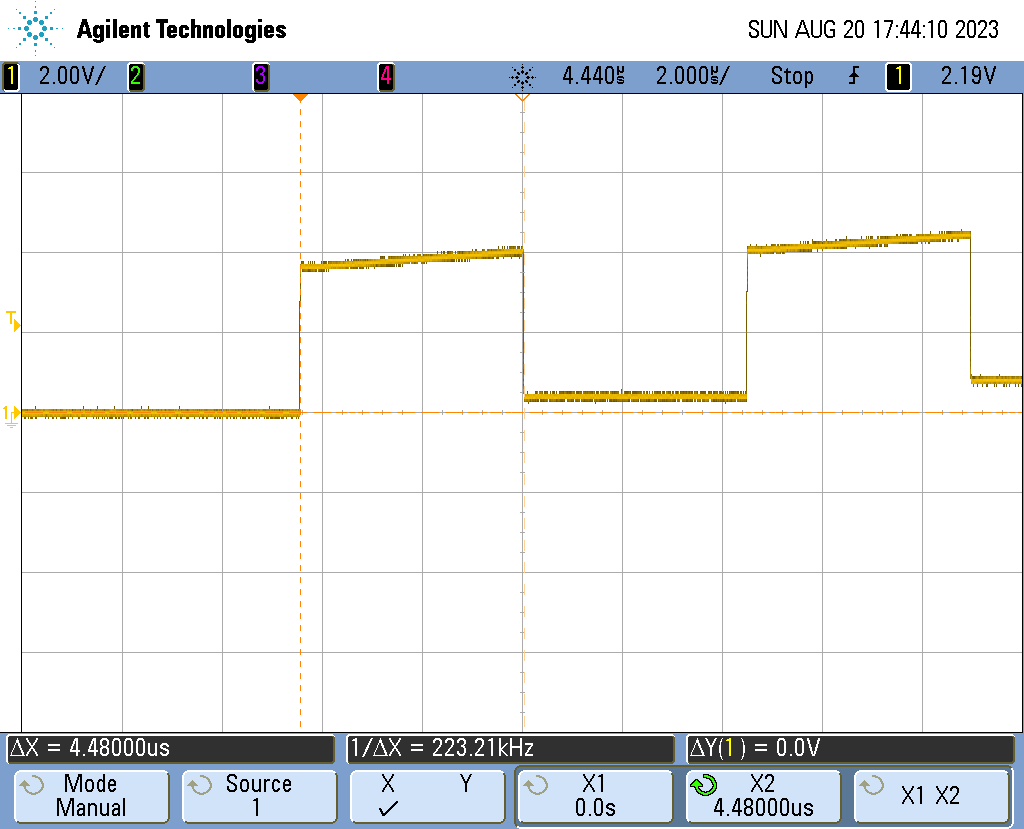
\includegraphics[width=0.75\textwidth]{Images/scope_4.png}
    \caption[Added latency by packet filter waveform]{Added latency by packet filter waveform.}
    \label{fig:packet_classifier_architecture}
\end{figure}

There is two pulses in this graph. This is due to when the crs\_dv line gets disasserted at the end of the packet. From this the time taken to receive the packet can be found to be 8.94uS. This is just an observation and is proportional to the packet size.



The same setup was used to test the preexisting solution, except this time GPIO pins were set high and low. It is assumed that the latency of setting the pin high cancels out with the latency of setting the pin low. 

\subsection{Limitations}
\subsubsection{PMOD Interface}

There are 5 PMOD connectors on the development board. Initally, one of these would be used for a second Ethernet PHY, but due to bandwidth limitations of the interface, the design had to be altered. The recommended bandwidth of these ports are 25MHz while the Ethernet RMII PHY would have been using 50Mhz signals over the interface. As such, signal integrity issues arose (see figure \ref{fig:eye_diagram}) and restricted the use to just one interface - the onboard PHY. A new development board with two PHYs would be needed.

\begin{figure}[h]
    \centering
    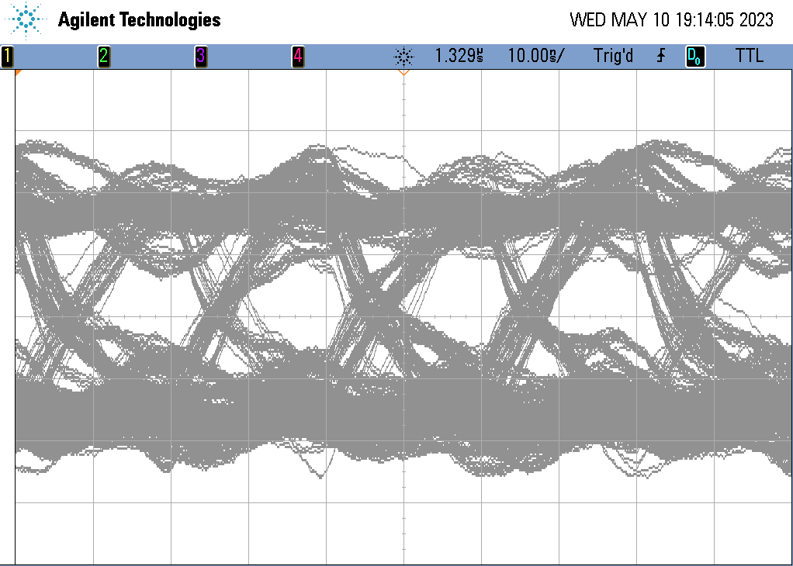
\includegraphics[width=0.65\textwidth]{Images/EyeDiagramTX.png}
    \caption[Eye diagram of TXD through PMOD interface]{Eye diagram of TXD through PMOD interface.}
    \label{fig:eye_diagram}
\end{figure}


\subsection{Testing setup}

\subsection{Results}



\section{Ultilisation}

The design can be broken down into several parts including the NeoRV32 processor itself, Ethernet and packet filtering hardware.

\begin{figure}[h]
    \centering
    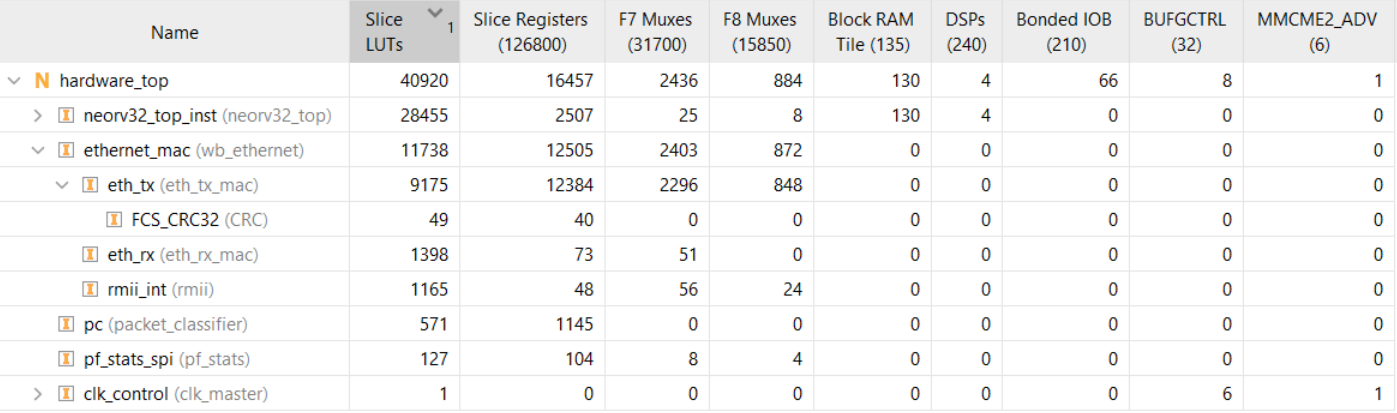
\includegraphics[width=0.85\textwidth]{Images/FPGAUtilisationResources.png}
    \caption[Summary of the resource utilisation on XC7A100T FPGA]{Summary of the resource utilisation on XC7A100T FPGA.}
    \label{fig:eye_diagram}
\end{figure}

The total number of resoruces on the FPGA are as follows: 63,400 LUTs, 126,800 flip flops, 135 BRAM tiles, 240 DSPs and 6 MMCMs.

LUT6 and LUT5 primatives were used the most in the design and by far the FDRE flip flop was the most used flip flop type. 2436 MUXF7s were also used. RAMD64E was also used in the design. The report from vivado can be found in appendix \ref{app:res_usage}.

\subsection{NeoRV32 processor}

The NeoRV32 SoC was configured to use the SPI, UART, GPIO, external interupts (XIRQ), true random number generator and importantly the wishbone B4 classic interface. The DSP48 blocks were used by the SoC to handle the multiply operations as this would free up LUTs and compute the result faster. 

The IMEM and DMEM sizes were chosen to consume as much of the remaining BRAM blocks left as possible. IMEM, the program storage was configured to 256KB while the DMEM, effectively the RAM, was configured to take the remaining amount left and set to 168KB in size. 

After synthesis of the design at 50Mhz, it was deemed that there was some headroom in the critical path delays. Hence the design was updated to 80MHz. This however does not affect the resource utilisation except for taking up some extra clock buffers. A single MMCM was still used to add the additional 80MHz output. 

The NeoRV32 itself took 28455 slice LUTs, 2507 Slice registers, 130 Block RAM tiles and 4 DSPs. 


\subsection{Ethernet hardware}
Comparatively, the Ethernet hardware took 11738 Slice LUTs and 12505 Slice registers, most of which is consumed by the transmit logic. This is largely due to the required buffers when storing (to construct) and sending out the frame. 

\subsection{Packet filter}
The packet classifier took a total of 571 Slice LUTs and 1145 Slice registers. This is lower than expected and indicates that the design could easily be increased to consolidate more rules. However, the fanout of the design will need to be considered due to the nature of the implementation. 





\section{Timing Summary}
\label{sec:timing_summary}
After running the post synthesis timing summary in Vivado, a worst negative slack of -2.634ns was reported for the setup timing with a total of 82 endpoints failing the constraints. For the hold summary, a worst hold slack of -0.021ns was found. 

The critical path is from the wishbone interface to the BRAM block inside the ethernet hardware - seen in figure \ref{fig:crit_path}. The level is 3 and stems from the NeoRV32 processor's wishbone bus. This cannot be easily updated and so is the leading limitation in the speed of the design. Even though this, in practice, doesn't seem to cause any issues, a caution for reliabilty is raised. 

\begin{figure}[h]
    \centering
    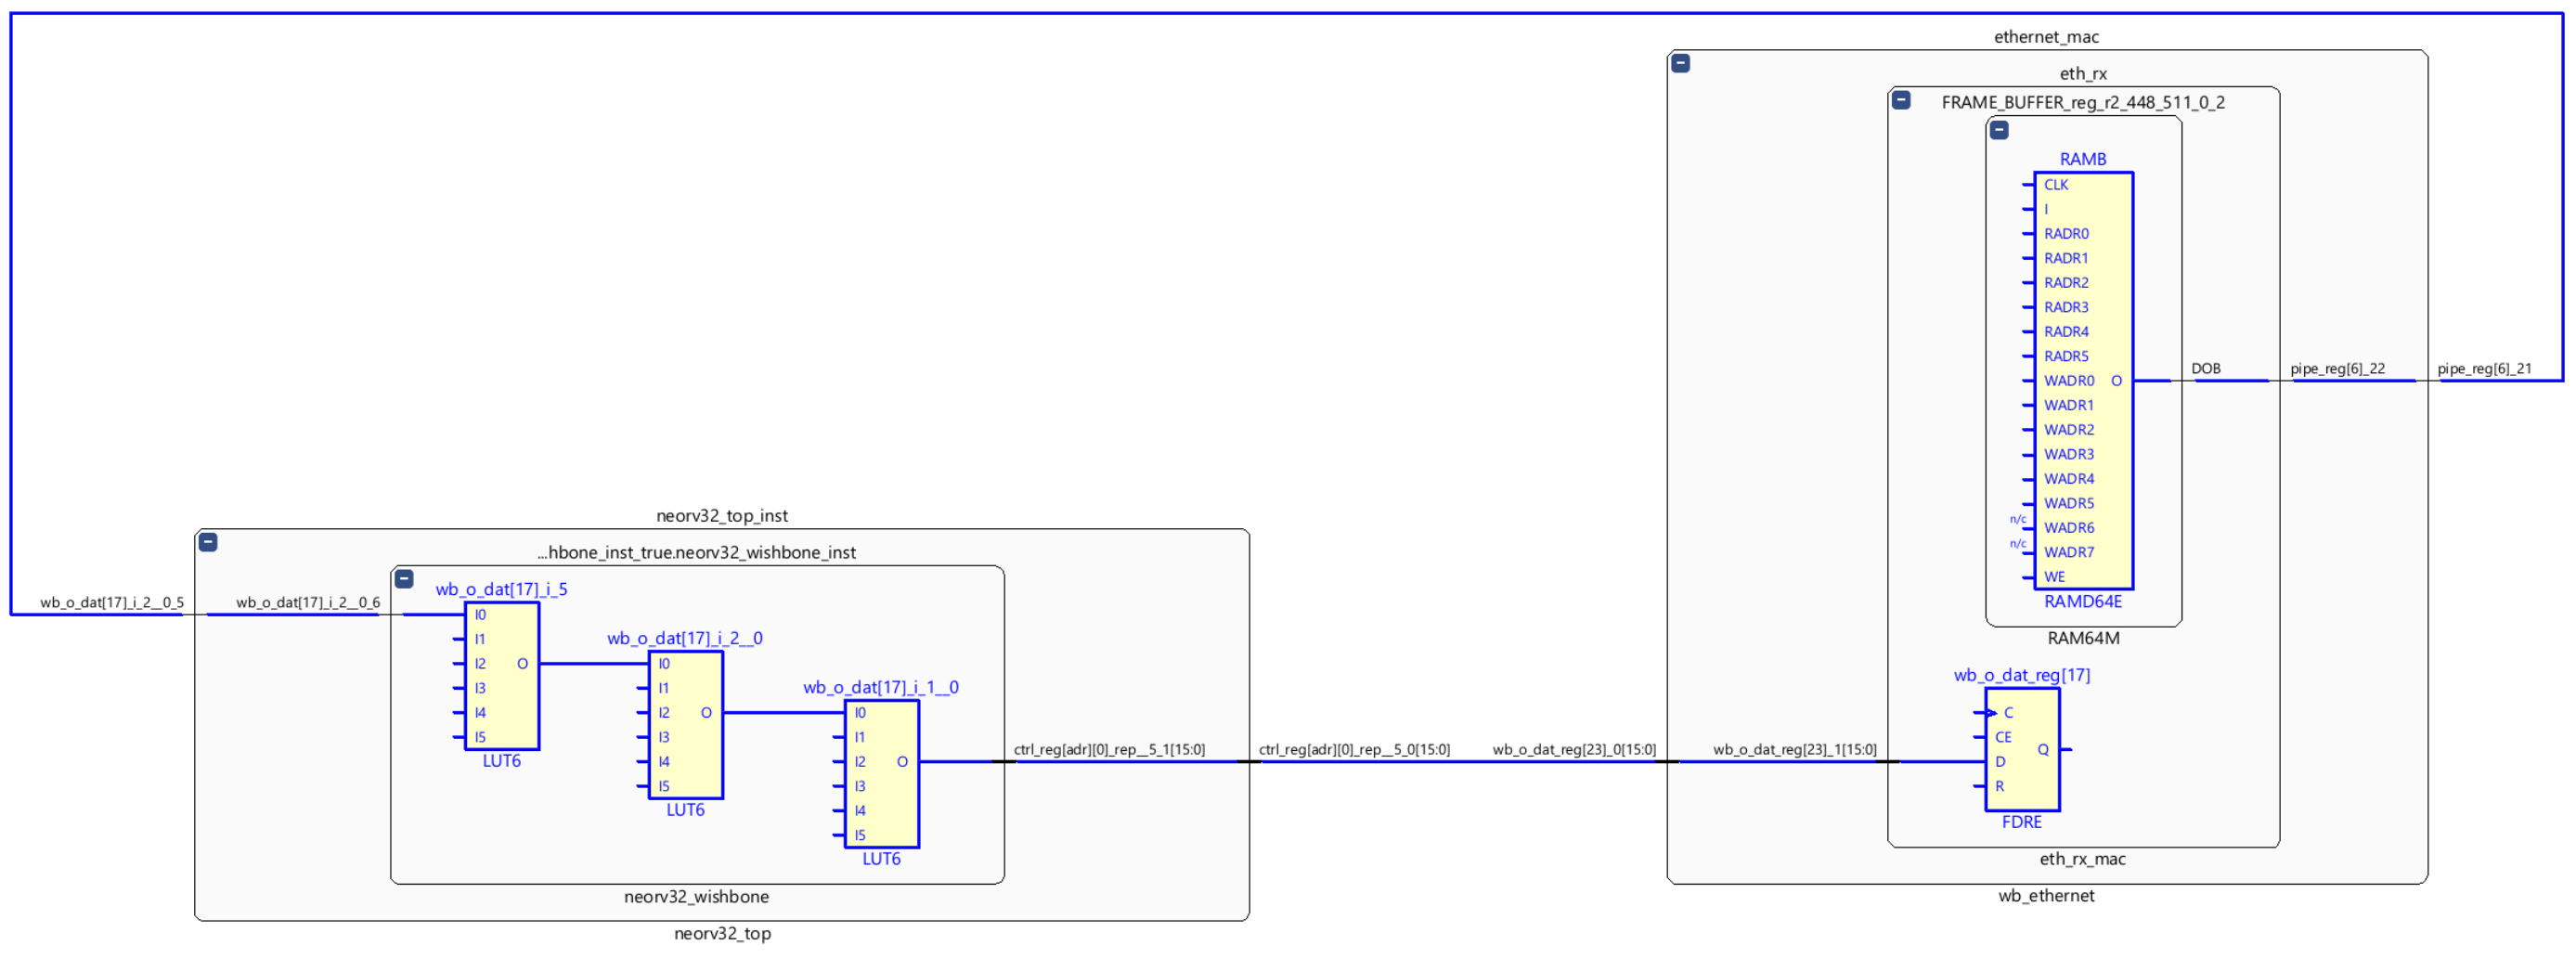
\includegraphics[width=1\textwidth]{Images/critical_path_delay_schematic.png}
    \caption[Critical path in SoC design]{Critical path in SoC design.}
    \label{fig:crit_path}
\end{figure}





\section{Comparison to preexisting solutions}


my solution is less suseptible to power glitch attacks since this is done at the hardware layer and not in software where instructions can be skipped. 
More secure and harder to bypass.
faster

Testing with WIZ5500 Pico, avg udp rtt was 1.88ms from 1000 tests with a payload of 7 bytes.
Testing with WIZ5500 Pico, avg udp rtt was 2.07ms from 1000 tests with a payload of 256 bytes.

Testing with LwIP Nucleo-F767ZI at 80Mhz, avg udp rtt was 1.41ms from 1000 tests with a payload of 7 bytes.
Testing with LwIP Nucleo-F767ZI at 80Mhz, avg udp rtt was 1.51ms from 1000 tests with a payload of 256 bytes.

Testing with LwIP Nucleo-F767ZI, avg udp rtt was 1.30ms from 1000 tests with a payload of 7 bytes.
Testing with LwIP Nucleo-F767ZI, avg udp rtt was 1.39ms from 1000 tests with a payload of 256 bytes.


Testing with FPGA board, avg udp rtt was 1.45ms from 1000 tests with a payload of 7 bytes.
Testing with FPGA board, avg udp rtt was 1.72ms from 1000 tests with a payload of 256 bytes.



\subsection{Thermal analysis}

A thermal camera was used to record the temperatures periodically. At an ambient room temperature of $24.8\degree C$ throughout the test, after 5mins the WIZ5500 ethernet chip heated to $58.0\degree C$ and RP2040 was at $46.6\degree C$. While the FPGA was at $38.0 \degree C$. This is a bit of an unfair comparison as the physical size of the FPGA is much larger than the WIZ5500. After two hours of constant UDP ping requests to both devices, figure \ref{fig:thermal_2hr} shows the FPGA board and WIZ5500 board's temperature gradient. The FPGA plateaued to a maximum of $40.4 \degree C$ while the WIZ5500 was $1.c \degree C$ cooler at, $56.8 \degree C$. This could be due to accuracy of the measurements, in addition to not getting aiming the thermal camera in the hottest part. The RP2040 chip however was measured to be $53.2 \degree C$. Some additional thermal images can be found in the appendix.


\begin{figure}[h]
    \centering
    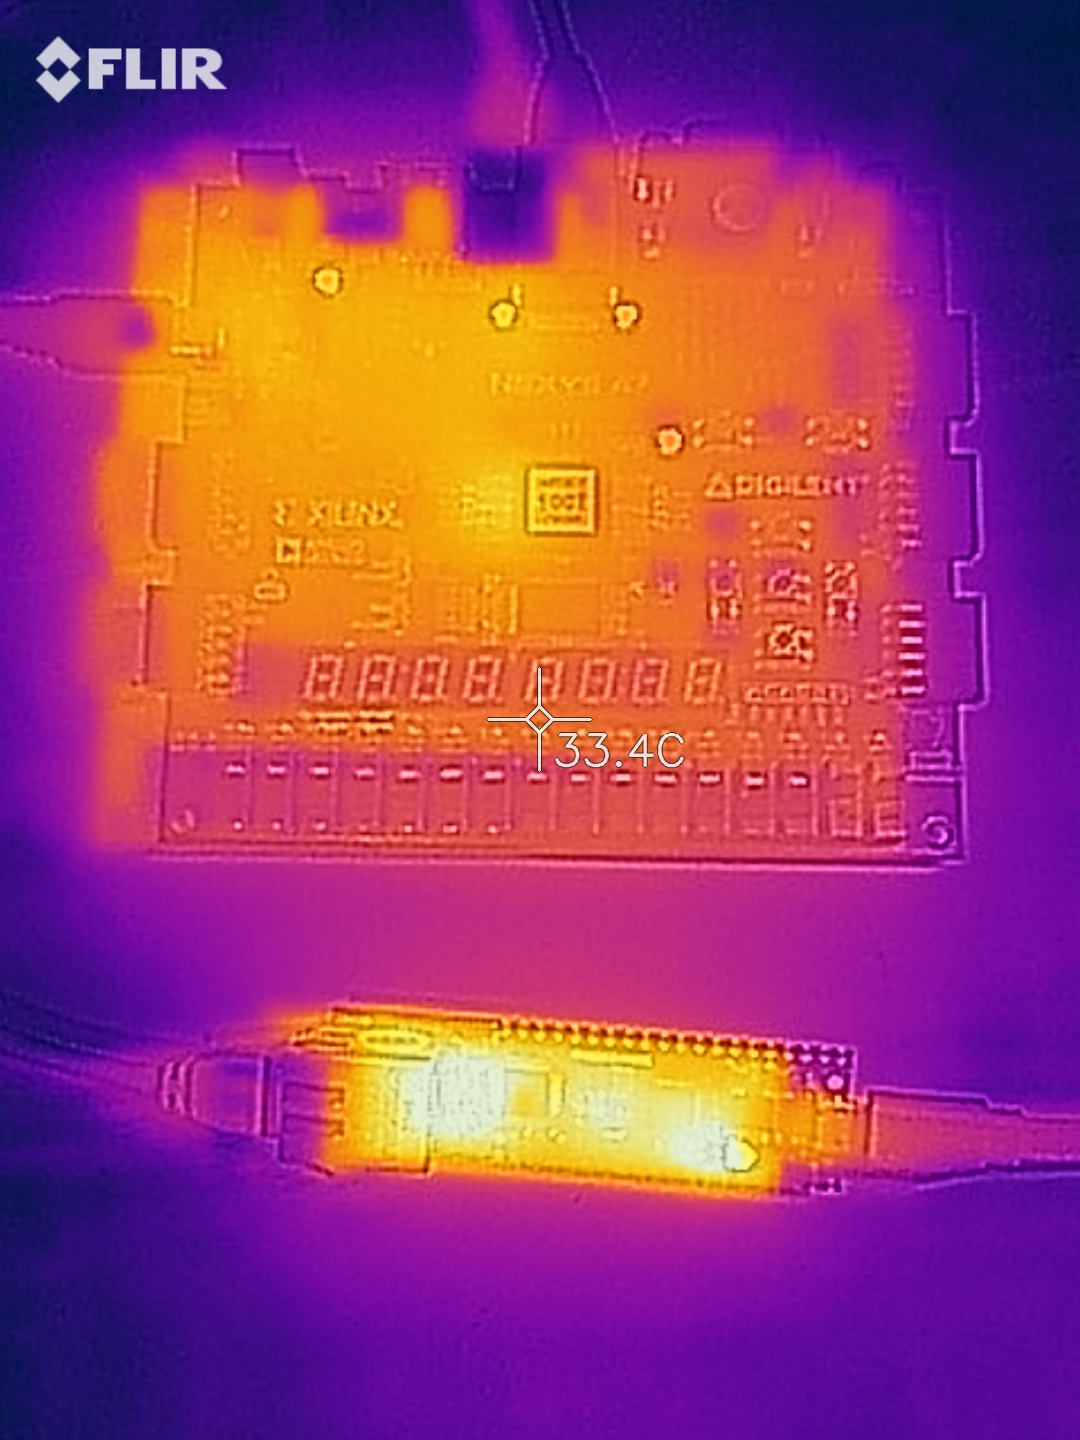
\includegraphics[width=0.5\textwidth]{Images/flir_2hs.jpg}
    \caption[Thermal image of FPGA board and WIZ5500 after two hours]{Thermal image of FPGA board and WIZ5500 after two hours.}
    \label{fig:thermal_2hr}
\end{figure}


\section{Power analysis}

As the voltage would remain constant between devices (all powered over USB), only the current was measured. These results however should be taken with caution as they do not account for regulator inefficiencies and do not give a true current reading of the device, rather just an indication. 


The device for testing the current was the Nordic Semiconductor Power Profiler Kit 2 which can record at up to 100kSa/s. For the tests in this report, only a sampling rate of 10kSa/s was used as it produces less noisy results. 

As a baseline, the Nexys A7 board draws 200mA with no design applied and is due to all the additional components on the board. With the design loaded up but without the processor flashed, the board took 284.4mA. After flashing the board, the idle current reached an average of 301.84mA.

A series of tests were then done and the currents were measured. By pinging the device every 50ms, the average current consumption was 300.72mA. Interestingly, the current consumption was cyclic similar to what is shown in figure \ref{fig:ppk_icmp_ping}. A UDP ping test was conducted and had an average current draw of 301.13mA. In both the ICMP and UDP pings, the current consumption was of similar style where the variance of the current was about 10mA. 


If the packets are now blocked by the filter, more about the design in terms of power consumption can be learned. After adding a rule in the packet filter, very little could be observed in the current consumption over the unblocked case. The same cyclic pattern in figure \ref{fig:ppk_udp_ping} could be seen. An average of 300.92mA was been consumed by the device and is within the margin of error of the device. Figure \ref{fig:ppk_icmp_ping} shows the that the period for the current waveform is about 83ms, which is much larger than the 50ms between pings to the device. After filming the status LED on the PHY output at 240 frames per second, the period of the LED was 20 frames equivalent to $\approx 84ms$ which aligns with the current measurements. 


\begin{figure}[h]
    \centering
    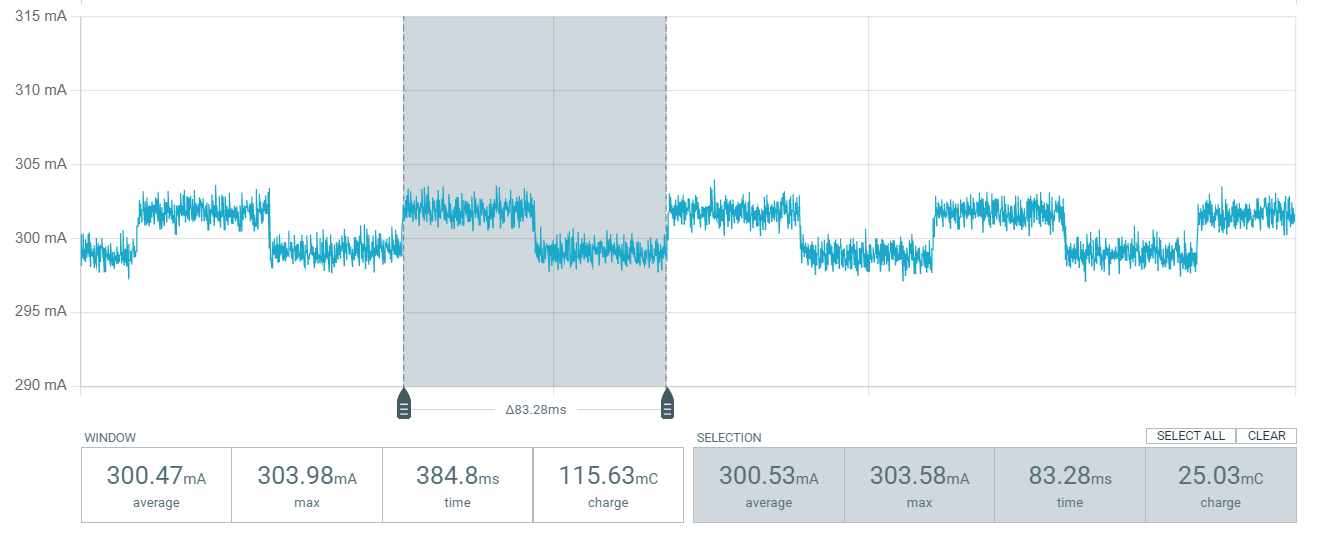
\includegraphics[width=0.9\textwidth]{Images/PPK_ping_zoom.png}
    \caption[Zoomed in current consumption for ICMP pings]{Zoomed in current consumption for ICMP pings.}
    \label{fig:ppk_icmp_ping}
\end{figure}



The next test was done when accessing the webserver. Figure \ref{fig:ppk_http_annotated} shows 5 different regions where each region is a result of a different action. The left most tests is from the inital HTTP requests to get the index page. Notably, there is 2 separate sections here, this is because the client fetches the html, css and favicon first and then requests the main (and much larger) javascript file after. The readings for each of these points is given as: average current, maximum current and time going from top to bottom. 

The second test is what happens when you click to navigate to the about page. The third event is when navigating to the config page and the 4th event is what happens when you press the 'load rules' button. The final test case is a refresh on the main page for the statistics. Notably, as the javascript (thus client) is doing the routing and page handling, future requests to get the contents of the pages are not needed, but only small API requests to update the data. Coincidentally, these first 3 requests also trigger a SD card read and explains the higher current draw. The fourth request also creates a read request to the SD card, but only needs to read a single page. The fifth request does not involve a read or write to the SD card, but rather just a simple SPI transaction takes place and consequently doesn't draw much additional power. 

\begin{figure}[h]
    \centering
    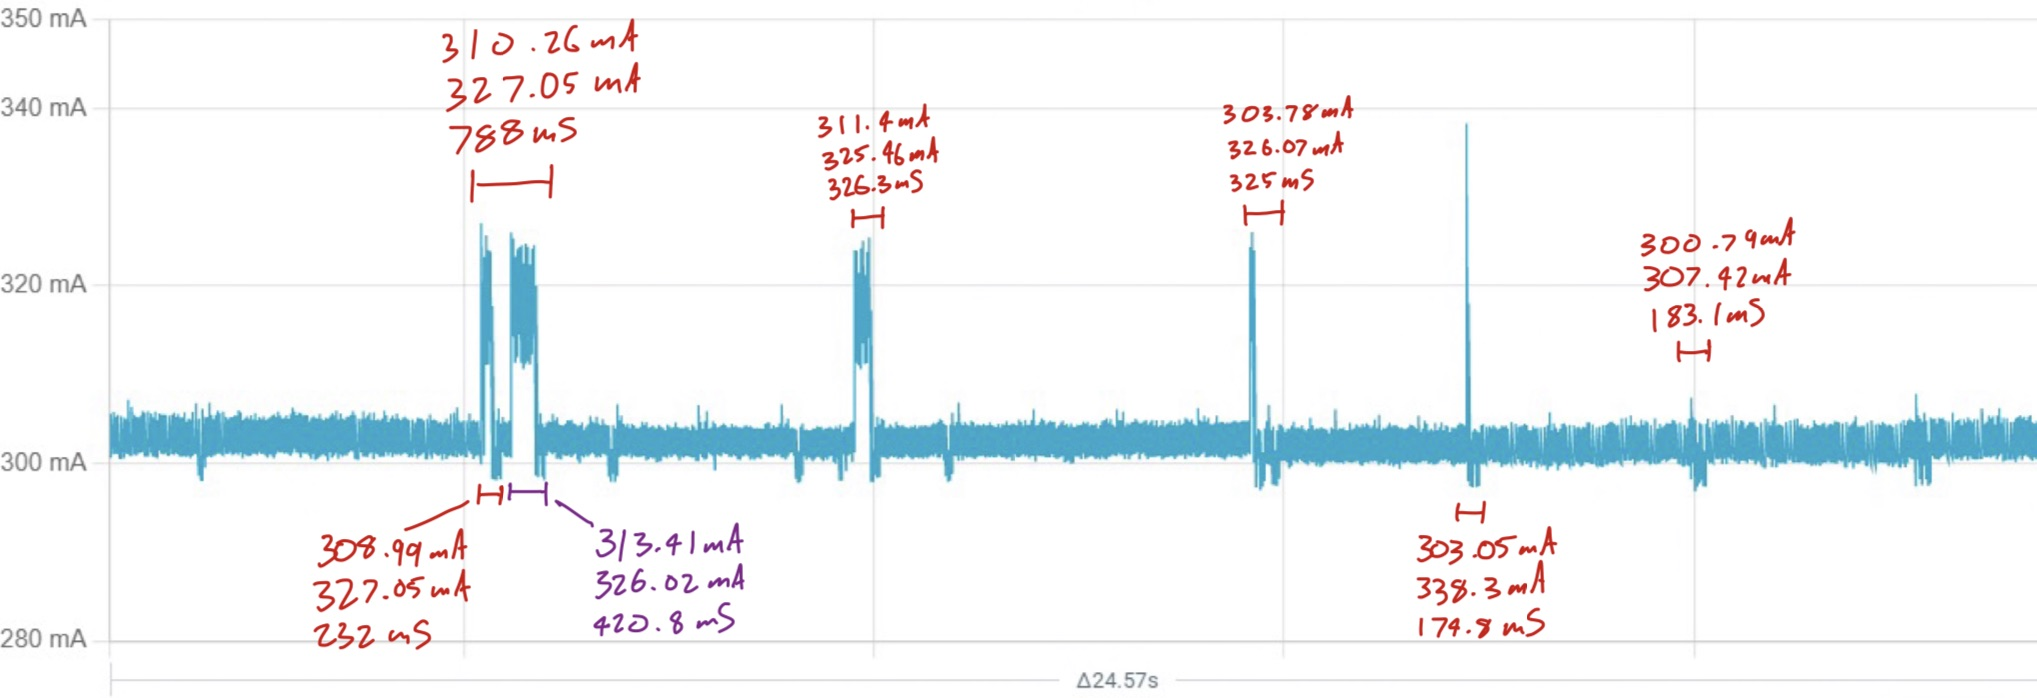
\includegraphics[width=0.9\textwidth]{Images/PPK_http_annotated.png}
    \caption[Current consumption of FPGA board with HTTP requests]{Current consumption of FPGA board with HTTP requests.}
    \label{fig:ppk_http_annotated}
\end{figure}


